
%!TEX ROOT=main.tex


\part{Software}
\label{chap:software}
\section{Introduction}
The control program for both the transmitter and the car is written in C language. It utilizes the STM32 HAL (Hardware Abstraction Layer) libraries, and the STM32CubeMX graphical utility was used to set up the necessary initialization and project files and generate code for peripheral configuration. Afterward, the application is compiled using a Makefile under Linux by the GNU GCC cross-compiler for ARM bare-metal targets.

STM32 HAL driver library provides a set of APIs to simplify interaction with all the peripherals and thus the user application implementation. The HAL driver layer implements run-time failure detection to increase robustness. HAL APIs are available for all peripherals. Also, the API ensures high portability across different STM32 families \cite{hal}.

STM32CubeMX is a graphical tool that provides a convenient user interface to configure the microcontroller. It allows a simple configuration of pin assignments, peripherals, or the clock tree, and the corresponding C initialization code generation. It also packs middleware stacks, such as USB, FatFs, or TCP/IP. This tool notably speeds up the process of microcontroller configuration and allows the user to focus on the application \cite{cubemx}.

The control program is almost exclusively interrupt-driven. Emphasis has been placed on program execution speed to ensure a high frequency of control commands and thus smooth car control.

\section{File structure}
Software for both the transmitter and car is in their respective folders. STM32CubeMX generated the code, and to maintain compatibility, the dedicated user code sections were used. The code was generated with CubeMX's basic application structure setting.

Therefore, both project folders in the \textit{'Software'} folder contain the \textit{'Drivers'} folder with ARM and HAL drivers for the board, the \textit{'Inc'} folder with header files, and the \textit{'Src'} folder with source files. The startup file, makefile, linker script, and CubeMX project file are in the root folder. As the car implements FatFs driver, it is located mainly in the \textit{'Middlewares'} folder.

The \textit{'shared\_libs'} folder contains shared libraries for both applications, namely the nRF24 module and OLED display libraries, and follows the same file structure; the \textit{'Inc'} folder contains header files and the \textit{'Src'} folder source files. Icons used on the OLED display are in the dedicated \textit{'logos'} folder inside the \textit{'Inc'} folder.
\newpage
In addition, there are three important files:
\begin{itemize}
	\item \begin{description}
\item[\textit{'project\_tamiya.h'}:]
Shared header located in the \textit{'shared\_libs/Inc'} folder. It contains common libraries and \textit{'platform.h'} file. More importantly, it contains nRF24 communication settings, various macros, and shared function declarations, namely nRF24 and OLED wrapper functions and functions used for UART debug prints.
\end{description}

	\item \begin{description}
\item[\textit{'project\_tamiya.c'}:]
Source file located in the \textit{'shared\_libs/Src'} folder. It consists of function definitions from the appropriate header file.
\end{description}

	\item \begin{description}
\item[\textit{'platform.h'}:]
This header file is in both applications' \textit{'Inc'} folder, contains platform-specific macros and settings, and includes platform-specific headers.
\end{description}
\end{itemize}
The visualization of the file structure with highlighted important files is below.

\begin{forest}
  pic dir tree,
  pic root,
  for tree={% folder icons by default; override using file for file icons
    directory,
  },
  [Software
    [Car, label=right:Main folder of the car control application
    		[Inc
    			[platform.h, file
    			]
    		]
    ]
    [shared\_libs, label=right:Shared libraries for both applications
    		[Inc
    			[project\_tamiya.h, file
    			]
    		]
    		[Src
    			[project\_tamiya.c, file
    			]
    		]
    ]
    [Transmitter, label=right:Main folder of the transmitter control application
    		[Inc
    			[platform.h, file
    			]
    		]
    ]
  ]
\end{forest}

\subsection{Communication parameters}
Since the communication parameters must be equal in both the car and transmitter to establish the connection, they are placed in the shared \textit{'project\_tamiya.h'} header file.

The control packet payload size is only 4 bytes, and the ACK packet payload is only 3 bytes. In addition, 1 byte CRC is used. Payloads are described in figures \ref{tab:ctrl_payload} and \ref{tab:ack_payload}. CRC and other fields of the \textit{Enhanced ShockBurst} packet are not displayed.

\begin{figure}[ht]
\centering
	\begin{bytefield}[bitwidth=1.2em, bitheight=2em]{32}
        \bitheader{0, 8, 16, 24, 32} \\
        \bitbox{16}{Throttle} & \bitbox{16}{Steering}
    \end{bytefield}
    \caption{Control payload format}
    \label{tab:ctrl_payload}
\end{figure}
	
\begin{figure}[ht]
\centering
	\begin{bytefield}[bitwidth=1.5em, bitheight=\widthof{~\small$\frac{1}{2}$\unit{\celsius}~}]{24}
        \bitheader{0, 8, 16, 17, 24} \\
        \begin{rightwordgroup}{RTP \\  Header}
        \bitbox{16}{Battery voltage} & \bitbox{1}{\rotatebox{90}{\small$\frac{1}{2}$\unit{\celsius}}} & \bitbox{7}{Integer temperature}
    \end{bytefield}
    \caption{ACK payload format}
    \label{tab:ack_payload}
\end{figure}
\noindent
Bit 16 of the ACK payload is related to the trick described in \ref{sub:integers}.

The channel frequency is set to \SI{2515}{\MHz} to reduce interferences with the wi-fi signal, and the data rate is the lowest possible \SI{250}{\kilo\bit\per\second}. According to \cite{nrf_datasheet}, a lower air data rate gives better receiver sensitivity than a higher air data rate. Transmitting power is, on the other hand, the highest possible. This setup ensures the most extended potential range.


\section{Transmitter}
\subsection{Peripherals and pin configuration}
\label{sub:tx_conf}
\begin{figure}[h]
\centering
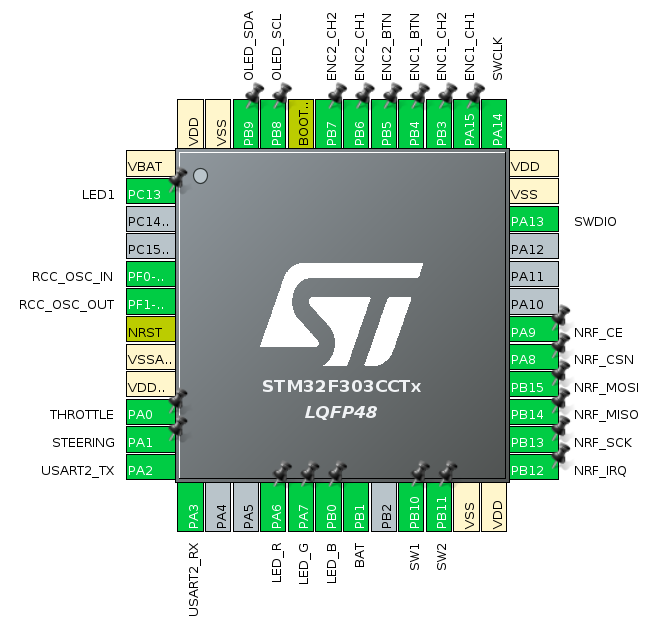
\includegraphics[width=0.7\linewidth]{fig/tx_pin_assignments.png}
\caption{Transmitter pin assignments}
\label{fig:tx_conf}
\end{figure}
\noindent
The microcontroller runs at \SI{72}{\MHz} with a clock source set to a \SI{12}{\MHz} external crystal oscillator.

ADC1 channels 1 and 2 are used to measure the output voltage from control potentiometers. ADC operates with 12-bit resolution in continuous conversion mode with DMA enabled in circular mode with continuous requests to manipulate the data. Once the ADC conversion is started, it remains active, and DMA repeatedly fills the buffer with measured data. Sampling time is the highest possible $601.5$ cycles, and software averaging is used to acquire stable measurements.

ADC3 uses channel 1 to measure the LiPo battery voltage and channel Vrefint to measure the internal reference voltage. Again, the resolution is 12-bit, continuous conversion mode is enabled, and DMA is utilized to transfer data from peripheral to memory. In this mode, the ADC remains active until DMA fills the whole data buffer. The sampling time for channel 1 is $601.5$ cycles, and for channel Vrefint $181.5$ cycles.

The communication module is connected to the SPI2 bus operating in full-duplex master mode. Baud rate is set to \SI{9}{\mega\bit\per\second}, and the data size is standard 8 bits. 'NRF\_IRQ' pin is configured in external interrupt mode with rising edge detection. The rest of the 'NRF' pins are simple outputs.

Quadrature rotary encoders utilize timers TIM2 and TIM4, which are in Encoder mode. This mode is designed specially to interface quadrature encoders with out-of-phase output signals. Encoder push-button pins are configured in external interrupt mode with rising edge detection.

SW1 and SW2 pins belong to the DIP switch and are configured in external interrupt mode with both rising and falling edge detection.

USART2 peripheral is configured as debug serial port. Baud rate is set to \SI{921600}{\bit\per\second} with 8~bits word length and one stop bit.

I2C1 in Fast Mode Plus with a frequency of \SI{1}{\MHz} connects the OLED display. LED pins are simple outputs. Furthermore, TIM6 at \SI{1}{\Hz} and TIM16 at \SI{4}{\Hz}, both timers with interrupts enabled, are used for basic timing purposes.

Figure \ref{fig:tx_conf} shows the complete pinout in STM32CubeMX.

\subsection{Application start}
The program starts with auto-generated initialization of all necessary peripherals. Debug UART is enabled after start by default. Afterward, an orange LED visible from the backside of the transmitter is turned on to indicate application initialization.

First, the OLED display is initialized, and the project logo is displayed. At the same time, a greeting is sent via UART, and the RGB LED flashes through each channel. Automatic self-calibration of both ADCs follows, and the Vrefint calibration value is obtained from the appropriate register. This value is later used to calculate VDDA. Then the communication module is initialized in transmitter mode with parameters defined in \textit{'project\_tamiya.h'}.

After that, the ADC responsible for reading values of control potentiometers is started in circular DMA mode, as described in section \ref{sub:tx_conf}. Processing of the data is explained in section \ref{sub:adc}.

In the final part of initialization, all the timers, including the timers used for quadrature encoders, are started in interrupt mode. Then the UART is deinitialized depending on the Switch1 state, the orange LED is turned off to indicate that initialization is done, and the program enters the main control loop.

\subsection{Main control loop}
The control loop is designed to be as non-blocking and interrupt-driven as possible. Therefore, it consists of a set of 'if' blocks. However, some parts remained blocking. The reason is some of the drivers are blocking and do not allow the use of DMA. Rewriting them was hardly possible or too time-consuming. This is especially true for OLED refreshing, which takes the longest time. Execution of given 'if' block is controlled by flags, internally boolean values, set by appropriate interrupt routines.
\newpage
\begin{itemize}
	\item \begin{description}
\item[\textit{'trigger\_data\_rdy'}:]
The flag is set by ADC interrupt routines and indicates available control values. This block processes and averages measured values from control potentiometers and recalculates them using hardware limits for direct usage in the car. The flag is reset at the end of the block.
\end{description}

	\item \begin{description}
\item[\textit{'adc\_data\_bat\_rdy'}:]
This block is similar to the previous block and indicates available voltage measurements.  First, it averages the measured $Vrefint_{meas}$ and battery voltage data. The next step is VDDA calculation:
\begin{equation}
	V_{DDA} = \frac{\SI{3.3}{\V} \cdot Vrefint_{cal}}{Vrefint_{meas}}\ ,
\end{equation}
where $Vrefint_{cal}$ is a value acquired during the manufacturing process at $V_{DDA} = \SI{3.3}{\V}$ and obtained from the register, and $Vrefint_{meas}$ is measured internal reference voltage. The formula was taken from Section 15.3.32 in \cite{f303_ref}. This computed value is used to convert the ADC battery measurement to the actual voltage.

The corresponding ADC sets the flag, and the program resets it at the end of the block. A~\SI{4}{\Hz} timer triggers the ADC measurement itself.
\end{description}

	\item \begin{description}
\item[\textit{'sending'}:]
This is the first phase of the non-blocking packet transmission routine. It is executed only if the flag is false, indicating that the previous transmission is completed. First, the flag is set, trimming values are added to the control values from potentiometers, and a 4-byte data packet is formed. After that, packet transmission is started. The flag remains set.
\end{description}

	\item \begin{description}
\item[\textit{'NRF\_IRQ'}:]
This is the second, final phase of the packet transmission routine. The communication module's interrupt pin sets the flag once it finishes the transmission. The routine starts with checking the transmission status and reading the received payload. If the payload has the expected size, it is parsed into related variables. Then actions depending on the transmission status follow.

The corresponding counter variable is incremented if the module has reached the maximum retransmit count. This variable is used to detect signal loss as described in section \ref{sub:tx_sig_loss}. If the transmission was successful, the previously mentioned variable is reset, the command frequency counter is incremented, and the status LED is toggled.

The last step is resetting both the \textit{'NRF\_IRQ'} and \textit{'sending'} flags.
\end{description}

	\item \begin{description}
\item[\textit{'display\_refresh'}:]
This section is responsible for refreshing the information on the OLED display. An interrupt routine of a \SI{4}{\Hz} timer sets the flag, and the program resets it at the end of the block. Therefore, the display runs with a framerate of about \SI{4}{FPS}.
\end{description}

	\item \begin{description}
\item[\textit{'ENCx\_IRQ'}:]
This section is executed when the rotary encoder's control timer triggers the interrupt routine upon detecting rotation. Depending on the direction of rotation, the trimming value is increased or decreased. The flag is reset at the end of the block.

Each encoder has its own control block modifying the appropriate trimming value.
\end{description}

	\item \begin{description}
\item[\textit{'ENCx\_reset'}:]
This flag is set by the encoder's push-button. The purpose is to reset the appropriate trimming value to zero. At the end of the block, the flag is reset.
\end{description}

\end{itemize}


\subsection{ADC data processing}
\label{sub:adc}
A feature similar to 'double buffering' is implemented to process data from ADC in circular mode. It is not implemented as two separate buffers but as a single 1024 bytes long buffer. It utilizes the ADC's ability to send notifications when the buffer is half-full and when it is full.

ADC is enabled and DMA starts filling the buffer with data. Once the buffer is half-full, the appropriate interrupt is triggered, and MCU is signaled to start processing the first half of the buffer. The DMA still fills the buffer with new data.

When the DMA fills the buffer completely, the appropriate interrupt is triggered, and the DMA starts filling the buffer from the beginning with new measurements. This state is again signaled to the MCU, which starts processing the second half of the buffer while the DMA fills the first half.

Whether the first or the second half is to be processed is controlled by an integer offset that is set in the interrupt routine. Hence, this method is fast as the DMA still fills the same buffer and does not need to be reconfigured, which would add additional overhead.

This approach is repeated, ensuring that the new measurements do not overwrite the values already in the buffer and, therefore, do not affect the value obtained.

\subsection{Signal quality and loss detection}
\label{sub:tx_sig_loss}
The nRF24 communication module does not support any detailed form of RSSI (Received Signal Strength Indicator). The only information obtainable from the module is whether the signal during the last transmission was below or under a certain threshold. Therefore, a simple signal quality indicator is implemented in the software.

After every successful packet transmission, the counter variable \textit{'tx\_freq\_cnt'} is incremented. During the callback routine of a \SI{1}{\Hz} timer, this value is copied into \textit{'tx\_freq'} variable and displayed. This value, expressing the number of packets per second, is used to measure the signal quality. Thresholds were determined experimentally based on the maximum observed number of packets per second.

Since the detection of signal loss by the transmitter is not as important as in the case of a car and serves mainly for information purposes, the implementation is quite simple.

It depends on the counter variable \textit{'retransmits\_in\_row'}, which is incremented whenever the communication module reaches the maximum number of packet retransmits and reset if the transmission was successful. When this variable is greater than 15, it is evaluated as a signal loss in the \SI{4}{\Hz} timer interrupt routine, and the corresponding flag is set.

This status is visualized on the OLED screen and by changing the color of the status LED to blue.

\subsection{Status visualization}
Both the RGB LED and OLED display are used to visualize the current status. The reasons for the choice are discussed in section \ref{sec:hw_status}.

The RGB LED is clearly visible and serves as a quick notification of the communication and the transmitter's battery status. Color options and their meaning are described in table \ref{tab:led_status}.
\begin{table}[h]
   \renewcommand{\arraystretch}{1.1}
   \centering
    \caption{Explanation of LED status}\label{tab:led_status}   
    \begin{tabular}{c c c}
       \noalign{\hrule height 1.1pt}\noalign{\smallskip}
	   \bfseries RGB LED & \bfseries Communication status & \bfseries Battery status\\[0.2em]
	\noalign{\hrule height 1.1pt}\noalign{\smallskip}     
flashing green	& OK				& $>\,$\SI{6.8}{\V} \\
flashing red		& OK				& $<\,$\SI{6.8}{\V} \\
blue				& signal lost	& --	\\
       \noalign{\smallskip}\noalign{\hrule height 1.1pt}
    \end{tabular}
\end{table} 

The small OLED display is more demanding for quick orientation in the displayed data. On the other hand, it provides more information about the transmitter and even the car. The display interface is divided into two main parts.

The first in the upper part of the display resembles a status bar and provides information about the car, as indicated by the icons: the BLDC temperature and battery state. In case of signal loss, this information is displayed here.

The rest of the screen is separated by a line and belongs to the transmitter status. Information about the current position of control potentiometers is displayed in the middle, along with the trim values. The position of potentiometers is not expressed relatively in percentage. Instead, the actual value sent to the car is displayed. The bottom part offers information about packets per second and the transmitter's battery status.

Both battery indicators are interactive and, depending on the voltage, up to 4 bars are displayed. If the battery voltage drops below the threshold of \SI{6.8}{\V}, a flashing exclamation mark is displayed in the battery logo instead. The signal quality indicator is also interactive.

All logos were created in GIMP and exported as XBM files. These were later 'converted' to header files by changing the file extension. Examples of the display interface are in figure \ref{fig:tx_oled}.
\begin{figure}[h]
    \centering
    \begin{subfigure}{0.35\textwidth}
    \centering
        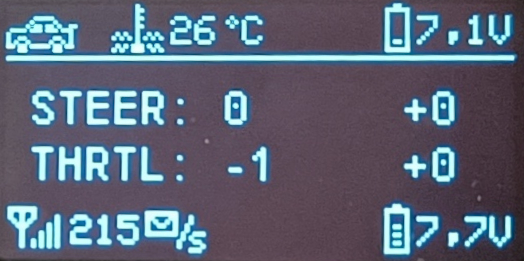
\includegraphics[width=1\textwidth]{fig/tx_oled_ok.jpg}
%		\caption{front side}
    \end{subfigure}%
    \hspace{1cm}
    \begin{subfigure}{0.35\textwidth}
    \centering
		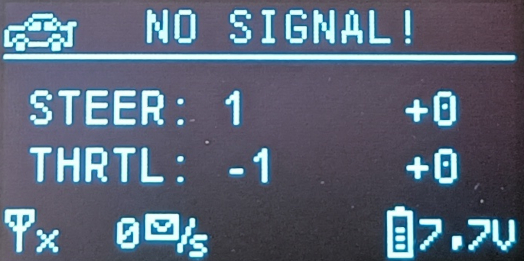
\includegraphics[width=1\textwidth]{fig/tx_oled_nosig.jpg}
%		\caption{back side}
    \end{subfigure}
	\caption{OLED display interface in transmitter}
    \label{fig:tx_oled}
\end{figure}

\subsection{UART debug prints}
One of the UARTs is utilized for printing debug information. Corresponding pins are available on the connector J3; configuration is in section \ref{sub:tx_conf}.

The printing is enabled by default after the application start and prints the initialization progress. Afterward, the printing is dependent on the state of the Switch1 (the first lever on the DIP switch SW2).

The UART is deinitialized before entering the main control loop if the switch is in the off position or stays initialized otherwise. If debug prints are enabled, the transmitter informs about:
\newpage
\begin{itemize}
\item LiPo battery voltage and VDDA voltage whenever new data is available,
\item encoder rotation,
\item switch position change,
\item no signal state.
\end{itemize}
Debug printing can be enabled or disabled anytime during the application execution.



\section{Car}
\subsection{Peripherals and pin configuration}
\label{sub:car_conf}
\begin{figure}[h]
\centering
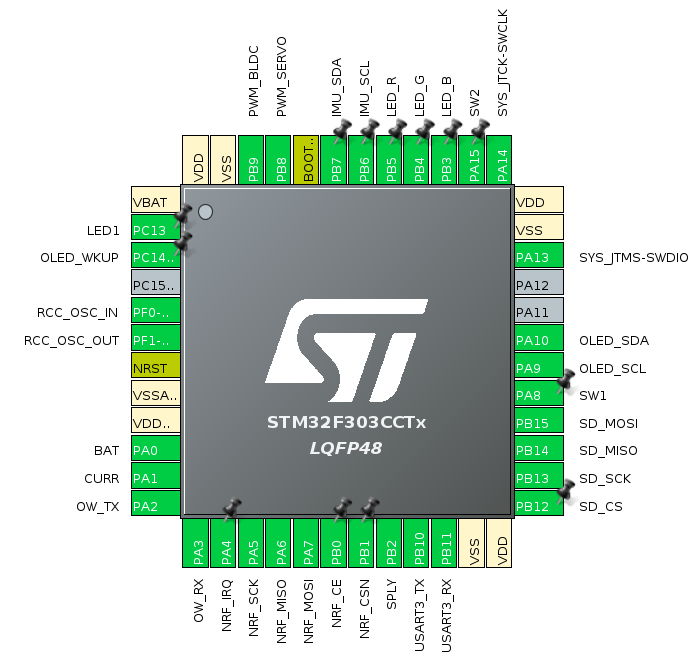
\includegraphics[width=0.75\linewidth]{fig/car_pin_assignments.png}
\caption{Car pin assignments}
\label{fig:car_conf}
\end{figure}
Some of the settings are similar to transmitter settings since both microcontrollers are the same STM32F303CCT6. The microcontroller runs at \SI{72}{\MHz} with a clock source set to an \SI{8}{\MHz} external crystal oscillator.

Channels 2 and 3 of timer TIM8 are used to generate PWM and therefore control the car. Prescaler and counter period values are calculated to represent the pulse width in microseconds. That means the counter value of e.g. $1500$ equals \SI{1500}{\micro\second} pulse width, which is convenient for control application implementation.

ADC1 channels 1 and 2 are used to measure the LiPo battery voltage and output voltage from the current sensor. ADC operates with 12-bit resolution in continuous conversion mode with DMA enabled. Sampling time is again the highest possible $601.5$ cycles to acquire stable measurements.

ADC2 measures the Vrefint channel to obtain the internal reference voltage and channel 12 to obtain the BEC output voltage. The resolution is also 12-bit, and continuous conversion mode with DMA is enabled. The sampling time for channel Vrefint is $181.5$ cycles and $601.5$ cycles for channel~12.

The communication module is connected to the SPI1 bus operating in full-duplex master mode. Baud rate is set to \SI{9}{\mega\bit\per\second}, and the data size is standard 8 bits. 'NRF\_IRQ' pin is configured in external interrupt mode with rising edge detection. The rest of the 'NRF' pins are simple outputs.

As STM32F303 does not support the SDIO interface, the SD card is connected via the SPI2 peripheral. The baud rate is only \SI{281.25}{\kilo\bit\per\second} after reset, but once the SD card is initialized, it is increased to \SI{9}{\mega\bit\per\second}.

I2C2 in Fast Mode Plus with a frequency of \SI{1}{\MHz} connects the OLED display. IMU unit is served by I2C1 in Fast Mode with a frequency of \SI{400}{\kHz}.

1-Wire bus necessary to communicate with the DS18B20 temperature sensor is implemented using USART2 peripheral and DMA. This method is described in \cite{1wire_uart}, and the DMA version was implemented with the help of \cite{1wire_uart_imp}. Since RX and TX pins are tied together, and TX pin is configured as push-pull, it is protected with a diode. This method is much simpler and requires fewer external components than the approach in \cite{1wire_uart} with a discrete open-drain buffer.

SW1 and SW2 pins belong to the DIP switch and are configured in external interrupt mode with both rising and falling edge detection.

USART3 peripheral is configured as debug serial port. Baud rate is set to \SI{921600}{\bit\per\second} with 8~bits word length and one stop bit.

LED pins are simple outputs. Pins PA11 and PA12 are not used in the project's current state but are reserved for a USB peripheral for possible future expansion with a control computer.

Figure \ref{fig:car_conf} shows the complete pinout in STM32CubeMX.

\subsection{Application start}
The application for controlling the car is written similarly to the transmitter. The program starts with the initialization of all peripherals. Debug UART is enabled after start by default, too, and a blue LED on the BlackPill board indicates application initialization.

First, the OLED display is initialized, and the project logo is displayed. At the same time and a greeting is sent via UART. If the Switch2 is turned on, IMU is initialized, and the flag controlling SD card logging is set. The next step is enabling servo and motor PWMs, initializing 1-Wire, and flashing individual channels of RGB LED.

Automatic self-calibration of both ADCs follows, and the Vrefint calibration value is obtained from the appropriate register. This value is later used to calculate VDDA. Then the communication module is initialized in receiver mode with parameters defined in \textit{'project\_tamiya.h'}.

After that, depending on the Switch2 position, the SD card is initialized and mounted. This process is explained in more detail in section \ref{sub:sd_log}.

Lastly, all the timers are started in interrupt mode. Timer TIM15 controlling the display timeout is immediately stopped afterward. This is because the timer triggers an interrupt when started for the first time even though it is not supposed to, which interferes with the display timeout feature.

Then the OLED display is turned off, UART is deinitialized depending on the Switch1 state, and the blue LED is turned off to indicate that initialization is done. The run time in milliseconds is stored just before entering the main control loop for possible later calculation of the data timestamp.

\subsection{Main control loop}
The following section describes the control loop. Similar to the transmitter control loop, it is designed to be as non-blocking and interrupt-driven as possible and consists of a set of 'if' blocks accordingly. The biggest bottleneck is the FatFs driver used for SD card logging, which is too complex to rewrite in DMA mode and takes the longest execution time. Individual 'if' blocks are controlled by their appropriate flag.

\begin{itemize}
	\item \begin{description}
\item[\textit{'NRF\_IRQ'}:]
The flag is set by the communication module and indicates the module's status change. If the status represents newly received data, an ACK packet is first prepared and sent back to the transmitter to confirm successful reception. If the received data has the expected size, processing follows.

Received values are checked against the defined chassis mechanical limits and clipped if they exceed the allowed range. After that, values are recalculated to pulse widths and set into PWM generating timers. Lastly, the safety timer is reset, and the command frequency counter is incremented. The flag is reset by the program at the end of the block.
\end{description}

	\item \begin{description}
\item[\textit{'temp\_conv\_ready'}:]
Although it may seem like the temperature sensor controls this flag, it is actually controlled by a \SI{1}{\Hz} timer. The temperature sensor datasheet states that temperature conversion with 12-bit resolution takes \SI{750}{\ms} and, therefore, one-second intervals are sufficient.

Nevertheless, this section indicates that the temperature conversion is done, and the reading process can be started. If SD logging is enabled, it also flushes cached data to the SD card with the \textit{'f\_sync'} function.
\end{description}

	\item \begin{description}
\item[\textit{'temp\_received'}:]
This is the section controlled by the temperature sensor. The flag is set by a~\mbox{1-Wire} interrupt and indicates that the measured data transfer from the sensor has finished. Thus the raw register data is converted to the actual temperature. The process is mentioned in section \ref{sub:integers}.

Lastly, the flag is reset, and the following temperature conversion is initialized.
\end{description}

	\item \begin{description}
\item[\textit{'adc\_data\_bat\_rdy'} and \textit{'adc\_data\_sply\_rdy'}:]
Appropriate ADC callback routines set flags. Both of them must be set to execute this block, which is responsible for processing data. First, measurements from both ADCs are averaged to obtain stable values. The VDDA calculation and conversion of values to the relevant physical quantities follows. Then if SD logging is enabled, data from IMU is read, and all the values are formatted and written to the SD card.

At the end of the block, both flags are reset. A \SI{50}{\Hz} timer triggers ADCs themselves.
\end{description}

	\item \begin{description}
\item[\textit{'log\_data'} and \textit{'unmount\_sd'}:]
This block ensures safe unmount and disconnection of the SD card. The file is truncated, closed, and the SD card is unmounted. If Switch2 is turned on after the start of the application, the \textit{'log\_data'} flag is set. The \textit{'unmount\_sd'} flag is set if it is turned off during execution. Both flags are reset at the end of the block.
\end{description}

	\item \begin{description}
\item[\textit{'display\_refresh'} and \textit{'display\_wakeup'}:]
This section is responsible for refreshing the information on the OLED display if it is turned on. An interrupt routine of a \SI{4}{\Hz} timer sets the \textit{'display\_refresh'} flag, and the program resets it at the end of the block. The \textit{'display\_wakeup'} flag is set for 5 seconds by pressing the push-button under the display, which also activates it.
\end{description}

\end{itemize}


\subsection{Integer arithmetics}
\label{sub:integers}
Although the selected MCU contains the FPU, all program variables are integers. The problem is not the speed of floating-point operations. Floating-point operations are fast thanks to the FPU and are used in some parts of the program, mainly during converting ADC value to actual voltage.

The problem is that formatting floats for output is slow and, in addition, requires a special flag for the linker and increases the final file size considerably. Hence, float variables are multiplied by~1000 to maintain at least some accuracy and saved as an integer. This approach applies mainly to the accelerometer data. The battery voltage value is already calculated in millivolts to avoid float variables altogether.

An easy 'trick' is utilized to display the BLDC temperature as a decimal number without float variables. The raw register data is converted to the integer part of the temperature using bits 11 to 4, according to Figure 4 in \cite{ds_datasheet}. Then the program checks the value of bit 3 associated with $2^{-1} = \frac{1}{2}$\unit{\celsius} and sets another integer variable to 5 or 0 accordingly. Afterward, the temperature is displayed as two integers with a point between them.

\subsection{Signal quality and loss detection}
\label{sub:safety}
It is expected from an RC vehicle that it safely stops or at least stops the motor in case of signal loss to prevent damage or injury. Since pulse width values controlling the servo and motor are only updated when a new control packet is received, loss of the signal would mean that the last command remains set in PWM generating timer and the car uncontrollably drives away.

One of the timers is used as a 'safety timer' to solve this behavior. The timer is set to \SI{4}{\Hz} with interrupts enabled, and its counter is reset whenever a command packet is successfully received. If no new command is received within \SI{250}{\ms}, the timer triggers an interrupt, resetting the motor and servo to their 'neutral' position and setting the \textit{'no\_signal'} flag. 

Moreover, the associated interrupt callback routine is the only one that directly interferes with car control, which ensures the motor is always reset after exactly \SI{250}{\ms} independently of the current program state if no new command is received.

Theoretically, one of the watchdogs could have been used instead of the timer as a more robust safety measure. However, not reloading it in time would mean restarting the MCU and interfering with SD card data logging.

The signal quality indicator is implemented identically to the transmitter. Each time the packet is successfully received, a counter variable is incremented. The value of the counter variable is copied to another variable and reset every second by a \SI{1}{\Hz} timer. This value is used to estimate signal quality, which is then visualized on the OLED display.

\subsection{SD logging}
\label{sub:sd_log}
A micro SD card slot is ready to use to record driving data. The application implements \textit{ChaN's} FatFs driver to interface the SD card, and therefore, any FAT-formatted micro SD card can be used. Driving data are saved with a frequency of \SI{50}{\Hz} in CSV file format.

The logged data includes a timestamp, voltage and current measurements, BLDC temperature, actuator control values, and IMU data. The exact format and corresponding units of quantities are always specified in the first two lines of the CSV file. An example of the data output is shown in figure \ref{fig:data_raw}.

Data logging is enabled if Switch2 is turned on during the application start. Unlike UART prints, it cannot be enabled anytime. Depending on the Switch2 position, the SD card mounting and preparation procedure is performed right after communication module initialization.
\begin{figure}[h]
\centering
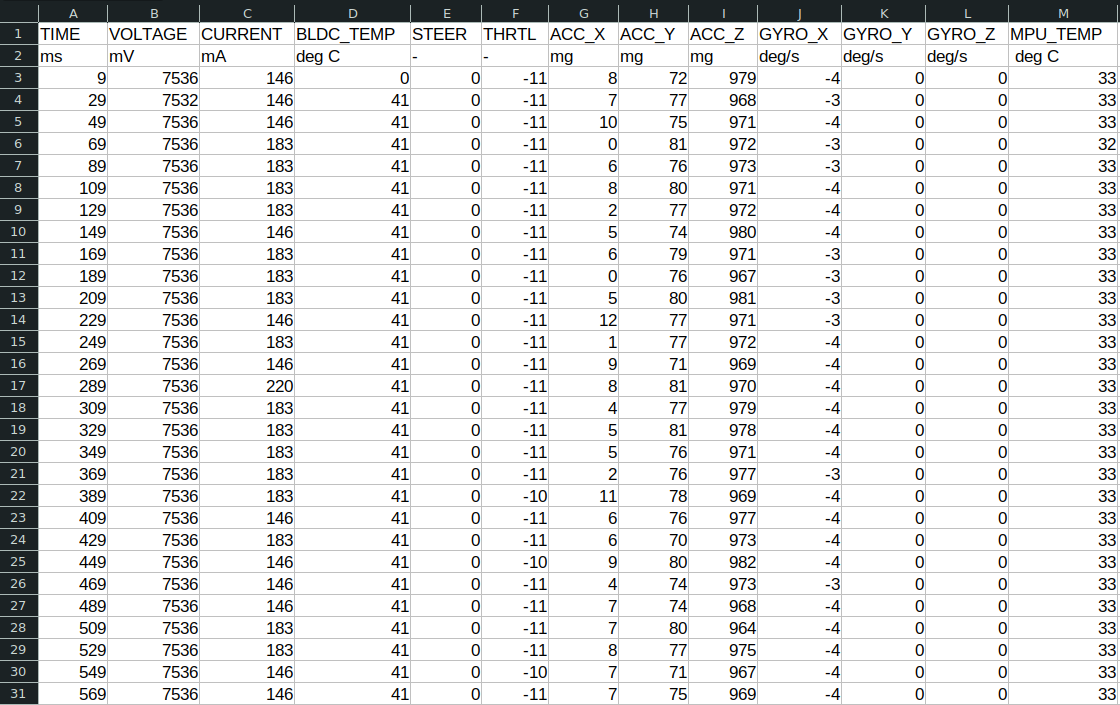
\includegraphics[width=1\linewidth]{fig/data_raw.png}
\caption{Example of raw data}
\label{fig:data_raw}
\end{figure}

It starts with mounting the disk and printing SD card statistics. Then the application search for the \textit{'logs'} folder, and if it is not found, it creates one. Afterward, the files in the folder are counted to determine the log number, and a new file is created.

Then pre-allocation of \SI{10}{\mebi\byte} of memory follows, which should suffice for approximately an \mbox{hour-long} log file. This step is critical as it dramatically decreases filesystem overhead when writing to the file. Without the pre-allocation, the \textit{'f\_sync'} function sometime took so long that the safety timer triggered and reset the motor.

Every second, the log file is \textit{'f\_synced'} to lower its execution time and prevent data loss if an unexpected event happens, such as a shutdown. With this approach, the user should not lose more than the last second of data.

Even though the pre-allocation reduced \textit{'f\_sync'} execution time significantly, it still sometimes takes more than \SI{100}{\ms}, meaning that some data are missing from the log.

Switch2 must be turned off to finish data logging properly. After that, the file is truncated and closed, and the whole SD card is safely unmounted.


\subsection{Status visualization}
Visualization of the status is consistent with the transmitter and utilizes the RGB LED and a bit smaller OLED display. Again, the RGB LED serves as a quick notification of the communication and the car's battery status. In the case of body shell mounting, it is also visible through it and is the only status indicator. The color scheme is the same as in the transmitter, and thus, the same table \ref{tab:led_status} applies.

Since the car is usually driven with a body shell mounted, the display is not visible to the user as it is under the body on the control board. For this reason, the display is turned off the majority of the time. It is activated only during the start of the application to display the project logo. The display can be turned on anytime by pressing the push-button under the display, waking it up for 5 seconds.

The display interface is much more plain than the one in the transmitter. 
Due to the size of the display, the only information presented is the battery voltage, motor temperature, and signal quality indicator with packets per second. Both battery and signal indicators are interactive again.

The signal loss is visualized only by the RGB LED and the zero frequency of the commands on the OLED display; no dedicated error message is shown. Examples of the display interface are in figure \ref{fig:car_oled}.
\begin{figure}[h]
    \centering
    \begin{subfigure}{0.4\textwidth}
    \centering
        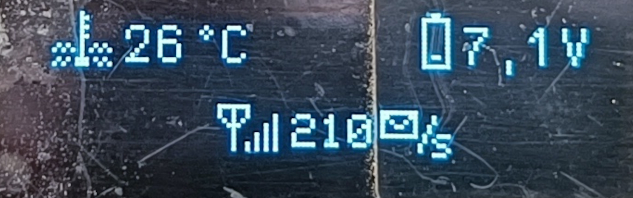
\includegraphics[width=1\textwidth]{fig/car_oled_ok.jpg}
%		\caption{front side}
    \end{subfigure}%
    \hspace{1cm}
    \begin{subfigure}{0.4\textwidth}
    \centering
		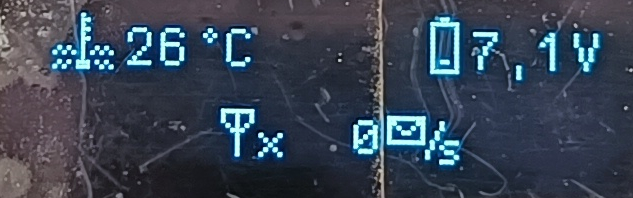
\includegraphics[width=1\textwidth]{fig/car_oled_nosig.jpg}
%		\caption{back side}
    \end{subfigure}
	\caption{OLED display interface in car}
    \label{fig:car_oled}
\end{figure}

\subsection{UART debug prints}
One of the UARTs is reserved for printing debug information. Corresponding pins are available on the pin header under the display; configuration is in section \ref{sub:car_conf}. The behavior is the same as in the transmitter.

The printing is enabled by default after the application start and prints the initialization progress. Afterward, the printing is dependent on the state of the Switch1.

The UART is deinitialized before entering the main control loop if the switch is in the off position or stays initialized otherwise. If debug prints are enabled, the car informs about:
\begin{itemize}
\item LiPo battery voltage and current, VDDA voltage, \SI{5}{\V} supply voltage, and BLDC temperature whenever new data is available,
\item file sync, save, write error if SD logging is enabled,
\item switch position changes and push-button presses,
\item no signal state.
\end{itemize}
Debug printing can be enabled or disabled anytime during the application execution.